\documentclass[12pt]{extarticle}
\usepackage[utf8]{inputenc}
\usepackage{cite}
\usepackage{blindtext}
\usepackage{graphicx} % Package to manage images
\usepackage{wrapfig} % Package to wrap text around figures
\usepackage{physics} % For the bra-ket notation.
\usepackage{amsmath} % For centering equations.
\usepackage{hyperref}
\usepackage{tikz}
\usetikzlibrary{quantikz}
\usepackage{pgfplots}
\usepackage{fancyhdr}
\usepackage{lastpage}

\pagestyle{fancy}
\fancyhf{}

%\rfoot{Page \thepage \hspace{1pt} of \pageref{LastPage}}

\hypersetup{
	colorlinks=true,
	linkcolor=blue,
	filecolor=magenta,      
	urlcolor=cyan,
	pdftitle={Name Of Experiment - Author Name},
	pdfpagemode=FullScreen,
}

\makeatletter

\renewcommand\paragraph{\@startsection{paragraph}{4}{\z@}%
	{-2.5ex\@plus -1ex \@minus -.25ex}%
	{1.25ex \@plus .25ex}%
	{\normalfont\normalsize\bfseries}}

\makeatother

\setcounter{secnumdepth}{4} % how many sectioning levels to assign numbers to

\setcounter{tocdepth}{4}    % how many sectioning levels to show in ToC


\fancyfoot[L,RO]{\thepage}

\chead{
\includegraphics[width=5cm, height=1cm]{./images/metu_logo.jpg}}



\begin{document}
	
	\clearpage
	%% temporary titles
	% command to provide stretchy vertical space in proportion
	\newcommand\nbvspace[1][3]{\vspace*{\stretch{#1}}}
	% allow some slack to avoid under/overfull boxes
	\newcommand\nbstretchyspace{\spaceskip0.5em plus 0.25em minus 0.25em}
	% To improve spacing on titlepages
	\newcommand{\nbtitlestretch}{\spaceskip0.6em}
	%\pagestyle{empty}
	\begin{center}
		\bfseries
		\nbvspace[1]
		\Huge
		{\nbtitlestretch\huge
			Compton Effect}
		
		\nbvspace[1]
		\normalsize
		
		\footnotesize  
		Author: Bartu Yaman
		\\
		Lab Partner: Riza Serkan Kaskan
		\\
		Experiment Date: 25.03.2022
		\\
		Submission Date: 01.04.2022
		
		
		
		
		\nbvspace[2]
		
		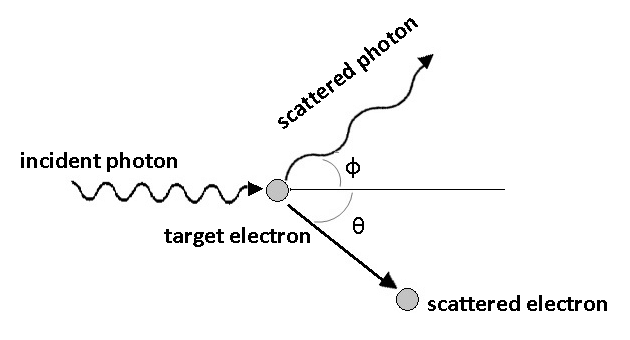
\includegraphics[width=3in]{./images/compton_effect.png}
		\nbvspace[3]
		\normalsize
		
		
		\nbvspace[1]
	\end{center}
	
	\newpage
	\tableofcontents
	\newpage
			
	\section{Introduction}

	\subsection{Goal}
		The goal of this experiment is to investigate the relation between the frequency of incident photons and the photocurrent. This relation will allow us to investigate the particle nature of light, helping us to understand the progression of modern physics and quantum theory through the years.
	
	\subsection{Theory}
		The underlying physical mechanism of photoelectric effect can be investigated under two different approaches. Going through the classical wave theory approach first is beneficial to understand the importance of the quantum theory.
		\subsubsection{Classical Theory Interpretation}
			In 1886, Heinrich Hertz realized that ultraviolet light can be used to eject electrons from a metal surface. 
			\\
			\\
			From the classical wave theory of light, the energy per unit volume for an electromagnetic wave can be written as:
			\begin{align*}
				u(x, t) = u_E + u_B = \frac{1}{2} \epsilon_0 E^2 + \frac{1}{2 \mu_0} B^2 
			\end{align*}
			This allows us to define the energy per unit area per unit time passing through a plane perpendicular to the wave, called the energy flux and denoted by $S$, which can be calculated by:
			\begin{align*}
				S = \frac{\text{Energy Passing Area A In Time t}}{\text{A * t}} = uc = \epsilon_0 c E^2 = \frac{1}{\mu_0} E B
			\end{align*}
			More generally, the flux of energy through any surface depends on the orientation of the surface. To take the direction into account, we introduce a vector $\vec{S}$, called the Poynting vector as:
			\begin{align*}
				\vec{S} = \frac{1}{\mu_0} \vec{E} \vec{B}
			\end{align*}
			The time average of the energy flux is the intensity $I$ of the electromagnetic wave $S_avg = I$. Therefore it is clear that the energy is proportional to the intensity of light according to this interpretation.
			\\
			\\
			The energy being proportional to the intensity (or the amplitude) according to the wave theory has some implications that conflict with the result of the photoelectric effect experiment. The problems with this intepretation are:
			\begin{itemize}
				\item The force applied to an electron is $F_E = eE$, which means that the force applied to an electron increases as the amplitude of the electric field, hence the amplitude, increases. This suggests that the kinetic energy of photoelectrons should increase as the intensity increases, which is not the case for the photoelectric effect. The maximum kinetic energy of photoelectrons are independent of are independent of light intensity.
				\item Wave theory suggests that the photoelectric effect should occur at any frequency, as long as the intensity if enough to excite the electrons on the surface of a metal. This contradicts with the existence of the cutoff frequency, $\nu_0$.
				\item The wave theory requires a time delay between the emission of light and the ejection of photoelectrons, but no such delay has been measured.
				\item The wave theory implies that the ejection of photoelectrons should be continuous since an electromagnetic wave is continuous. Which is not correct as it will be explained in the quantum theory. 
			\end{itemize}
		
		\subsubsection{Quantum Theory Interpretation}
			The "light quanta" hypothesis, which was hypothesized by Einstein in 1905, provided a revolutionary explanation to the photoelectric effect. Einstein proposed that light behaves as a stream of independent, localized units ,or quanta, of energy. 
			\\
			\\
			Then he proposed that a photon could be absorbed by transferring all of its energy to a single electron and that radiation itself consisted of packets of energy, which can be shown as:
			\begin{align*}
				h \nu = \frac{1}{2} (m v^2)_{max} + W_0
			\end{align*}
			where $W_0$ is the work function of the material. The work function is defined as the minimum thermodynamic work required to remove an electron from a solid and it can be shown as:
			\begin{align*}
				W = -e \varphi - E_F,
			\end{align*}
			where $-e$ is the electron charge, $\varphi$ is the electrostatic vacuum and $E_F$ is the Fermi level inside the solid where The term $-e \varphi$ signifies the rest energy of an electron in vacuum. In quantum systems, if the process is allowed by quantum mechanics, either all of the energy from a photon is absorbed or none of the energy of the photon is absorbed. This means that if the energy is not enough, i.e. the frequency is insufficient,  nothing will happen.
			\\
			\\
			The quantum theory is successful at explaining the existence of a cut off frequency as well. While observing the photoelectric effect, a positive external voltage is used to direct the photoemitted electrons onto the collector. If we use a negative voltage, it only allows the highest energy electrons to reach the collector. When there is no photocurrent, it means tat the negative voltage is enough to prevent the photoelectrons with the maximum kinetic energy $K_{max}$. This value of the voltage is called the cut off potential or the stopping potential $V_0$. When this value is reached, the work done by the cut off potential is enough to stop the electrons and this yields:
			\begin{align*}
				e V_0 = K_{max}.
			\end{align*}
			It is clear that the approach chosen by Einstein negated all of the shortcomings of the classical wave theory to explain the photoelectric effect. Einstein was also able to calculate Planck's constant really close to the value Max Planck obtained using the data from photoelectric effect experiments.
	
	 
	
	\section{Experimental Details}

	\subsection{Equipment}
		The experiment apparatus consisted of a mercury filled tube situated inside an electric oven, a thermocouple with its probe positioned just above the filled tube a power supply and an analog oscilloscope.
		\\
		\\
		The main apparatus had an electric oven to increase the collision probabilities of mercury atoms and incident electrons, a thermocouple connected to a digital thermometer to measure the temperature and a cathode ray tube filled with mercury to observe the actual phenomena. The power supply was specifically tailored for this experiment and allowed us to control the filament voltage, collector voltage and the accelerating voltage. The oscilloscope allowed us to get readouts from the apparatus, generating the same plot from Figure \ref{fig: fh}. 
	
	\subsection{Procedure}
	
		The procedure consisted of turning the thermostat dial to approximately 160 degrees Celsius (the temperature values were quite unstable, we tried not to exceed 200 degrees Celsius), setting the toggle switch to 'Ramp', setting filament to approximately 6 Volts, setting the collector voltage to approximately 2 Volts, adjusting the amplification gain, adjusting the oscilloscope variables to see clear and many peaks and writing down the data measured from the maximum and minimum values of the peaks present on the oscilloscope screen. 

	
	
	\section{Measurement And Data Analysis}

	\subsection{Presentation Of Data}
		\begin{table}[htbp]
			\centering
			\begin{tabular}{|c|c|c|c|c|c|c|}
				\hline
				\multicolumn{2}{|c|}{} &\multicolumn{5}{|c|}{Aperture: 4mm} \\
				\cline{3-7}
				\multicolumn{2}{|c|}{}  & $\lambda = 365nm$ & $\lambda = 405nm$ & $\lambda = 435nm$ & $\lambda = 546nm$ & $\lambda = 577nm$\\\hline
				
				\multirow{10}{*}{\rotatebox{90}{Data}}  & -2V & \(-3.4A\) &  \(-12A \)&  \(-11.1A\) &  \(-9.3A\) &  \(-3.7A\) \\\cline{2-7}    
				&-1.5V & \(209A\) &  \(3.2A\) &  \(-6.5A\) &  \(-9A\) &  \(-3.6A\) \\\cline{2-7}
				&-1.0V & \(637A\) &  \(101A\) &  \(104.7A\) &  \(-8.3A\) &  \(-3.5A\) \\\cline{2-7}
				& -0.5V & \(1084A\) &  \(236A\) &  \(316A\) &  \(98.3A\) &  \(22A\) \\\cline{2-7}
				& 0V & \(1600A\)&   \(385A\)&   \(540A\)    & \(350A\) &    \(125.2A\) \\ \cline{2-7}
				& 5V& \(8570A\) & \(2160A\)& \(3060A\)&   \(2040A\)&   \(721A\)\\\cline{2-7}
				& 10V& \(14600A\) & \(3660A\)& \(5180A\)&   \(3170A\)&   \(1141A\)\\
				\cline{2-7}
				& 15V& \(19670A\) & \(4860A\)& \(6800A\)&   \(4000A\)&   \(1401A\)\\\cline{2-7}
				& 20V& \(23700A\) & \(5900A\)& \(8250A\)&   \(4610A\)&   \(1577A\)\\\cline{2-7}
				& 25V& \(27300A\) & \(5900A\)& \(8250A\)&   \(4610A\)&   \(1577A\)\\\cline{2-7}
				& 30V& \(30200A\) & \(7480A\)& \(10400A\)&   \(5290A\)&   \(1790A\)\\
				\hline  
				
			\end{tabular}
			\caption{Experimental Data}
			\label{tbl:data}
		\end{table}
	
		\begin{figure}[H]
			\centering
			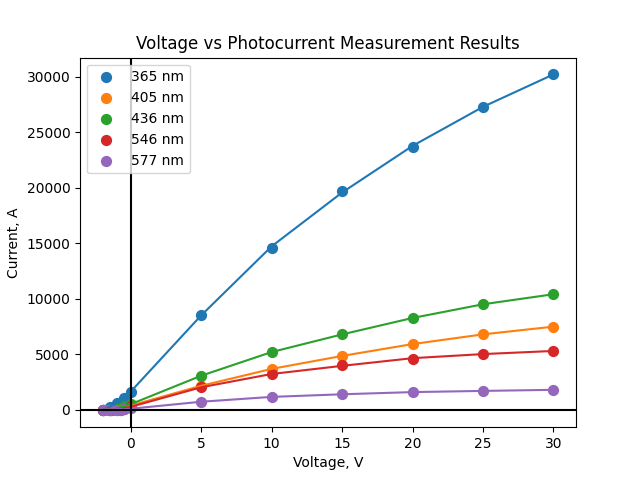
\includegraphics[width=10cm]{images/plot1a_pe.png}
			\caption{Voltage versus current plot of the data in Table \ref{tbl:data}.}
			\label{fig:pl1a}
		\end{figure}
	
		\begin{figure}[H]
			\centering
			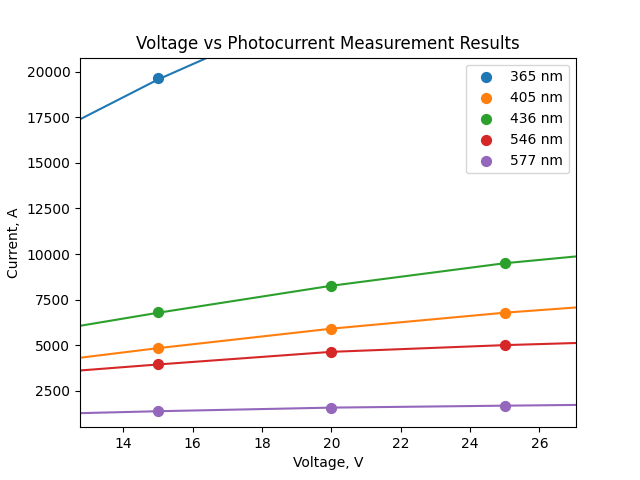
\includegraphics[width=10cm]{images/plot1b_pe.png}
			\caption{Voltage versus current plot of the data in Table \ref{tbl:data}, enlarged to highlight the difference in current.}
			\label{fig:pl1b}
		\end{figure}
	
		\begin{table}[htbp]
			\centering
			\begin{tabular}{ |l|l|l| }
				\hline
				\multicolumn{2}{ |c| }{Stopping Voltages, V: Current = 0A} \\
				\hline
				365 nm & -1.944 V\\ \hline
				405 nm& -1.55 V\\ \hline
				436 nm& -1.331 V\\ \hline
				546 nm& -0.784 V\\ \hline
				577 nm& -0.683 V\\ \hline
				
			\end{tabular}
			\caption{Stopping Voltage Data}
			\label{tbl:stpv}
		\end{table}
		
	
		\begin{figure}[H]
			\centering
			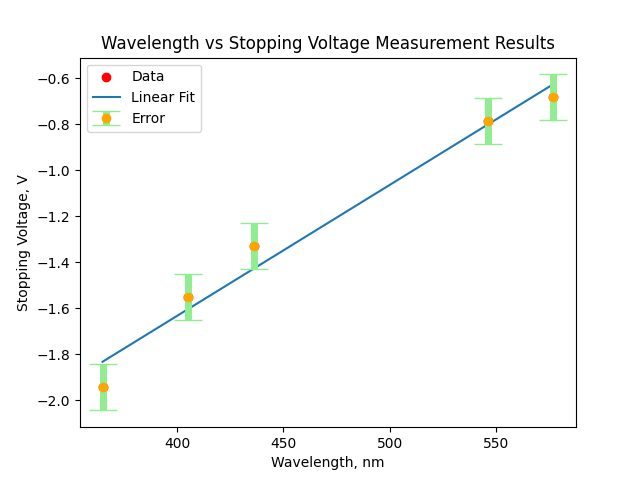
\includegraphics[width=10cm]{images/plot2_pe.png}
			\caption{Voltage versus current plot of the data in Table \ref{tbl:stpv}.}
			\label{fig:plt2}
		\end{figure}
	
	
	
	\section{Results And Discussion}

	\subsection{Results}
	Equation of the line in Figure \ref{fig:plt2} is $f(x) = 0.005695 x - 3.911$, which in physical context means that we have $V_s(\nu) = 0.005695 \nu - 3.911$. Multiplying this equation with electron charge $e$, we know that the resulting term needs to be equal to $KE_{max} = h \nu - \Phi$. 
	\begin{equation}
		V_s(\nu) e = KE_{max} \rightarrow 0.005695 \nu e - 3.911 e = h \nu - \Phi
	\end{equation}
	Then we obtain Planck's constant and the work function as:
	\begin{equation}
		h = 0.005695e \quad \text{ and } \quad \Phi = 3.911e
	\end{equation}
	\\
	\\
	In terms of errors, the phototube was isolated quite well from external light sources but it was quite apparent that there was some charge buildup inside the photoelectric effect experiment apparatus which forced us to re-calibrate it several times during the experiment to get consistent measurements.
	
	\subsection{Discussion}
	The validity of Einstein's theory was easily recognizable even without carrying out any calculations. Just looking at raw data was enough to say that photon energy depended on the wavelength of the incident photons but plotting the data and carrying out the calculations to validate the results with already established constants solidified this claim.
	
	
	\nocite{*}
	\bibliographystyle{plain} % We choose the "plain" reference style
	\bibliography{ref} % Entries are in the refs.bib file
			
		
\end{document}
